\documentclass[aps,twocolumn,secnumarabic,balancelastpage,amsmath,amssymb,nofootinbib, floatfix]{revtex4-1}
\usepackage[russian]{babel}
\usepackage{graphicx}      % tools for importing graphics
\usepackage{float}
\usepackage{epsf}          % old package handles encapsulated postscript issues
\usepackage{bm}            % special bold-math package. usge: \bm{mathsymbol}
\usepackage[colorlinks=true]{hyperref}  % this package should be added after 
\usepackage[inkscapelatex=false]{svg}
\usepackage{subfigure}
\usepackage{amsmath}
\usepackage{amssymb}
\usepackage{wrapfig}

	%%%%%%%%%%%%%%%%%%%%%%%%%%%%%%%%%%%%%%%%%%%%%%%%%%%%%%%%%%%%%%%%%%%
	% And now, begin the document...
	%%%%%%%%%%%%%%%%%%%%%%%%%%%%%%%%%%%%%%%%%%%%%%%%%%%%%%%%%%%%%%%%%%%
	\begin{document}
	\title{Объемная голограмма\\}
	\author{Лузгина А.А.}
	\email{luzgina.aa@phystech.edu}
	\homepage{\\https://old.mipt.ru/education/chair/physics/laboratornyy-praktikum/} %If you don't have one, just comment out this line.
	\date{\today}
	\affiliation{Столы, отчисленных соседей, ванная комната и ноутбук фирмы "Maxwell equations"}

	\begin{abstract}
		Работа представляет комплексное исследование голографии, сочетающее экспериментальную часть и программное моделирование. В экспериментальной части реализована запись голограмм по методу Денисюка с использованием пластин ПФГ-03М и лазерного источника. Разработана программная модель записи и восстановления голограмм Габора на основе численного моделирования интерференции и дифракции. Для точечных источников продемонстрирована корректная симуляция интерференционных паттернов и параллакса при смене ракурса. Выявлены проблемы при моделировании объёмных объектов, связанные с расчётом фаз, и предложены пути решения через декомпозицию на точечные источники. Экспериментально установлены оптимальные условия записи и выявлены ключевые факторы, влияющие на качество голограмм: вибрации, когерентность излучения и параметры экспозиции. 
	\end{abstract}
	
	\maketitle
	
	\section{Введение}  
	
	Голография — метод записи и воспроизведения трёхмерных изображений, основанный на интерференции когерентных волн. В отличие от традиционной фотографии, фиксирующей только интенсивность света, голография сохраняет информацию о фазе волны, что позволяет восстанавливать полное трёхмерное изображение объекта.  
	
	Данная работа сочетает экспериментальные исследования и компьютерное моделирование:
	\begin{enumerate}
		\item \textbf{Экспериментальная часть} посвящена записи голограмм по методу Денисюка с использованием:
		\begin{itemize}
			\item Голографических пластин ПФГ-03М (5000 штр/мм)
			\item Лазерного источника (длина волны 532 нм)
			\item Специализированных химических реактивов (проявитель OD1, фиксаж)
		\end{itemize}
		\item \textbf{Программное моделирование} реализует:
		\begin{itemize}
			\item Расчёт интерференционных картин для произвольных объектов
			\item Восстановление изображения методом БПФ
			\item Визуализацию с учётом положения наблюдателя
		\end{itemize}
	\end{enumerate}
	
	\section{Цели и задачи}  
	
	\textbf{Основные цели исследования:}
	\begin{enumerate}
		\item Реализовать экспериментальную запись голограмм объёмных объектов
		\item Разработать точную модель симуляции голограмм Габора
		\item Установить критические параметры, влияющие на качество записи
	\end{enumerate}
	
	\textbf{Конкретные задачи:}
	\begin{enumerate}
		\item \textit{Экспериментальные:}
		\begin{itemize}
			\item Оптимизировать схему установки для минимизации вибраций
			\item Определить оптимальное время экспозиции (10-20 сек)
			\item Проверить влияние фона и расстояний на качество записи
			\item Проанализировать причины неудачных попыток записи
		\end{itemize}
		\item \textit{Вычислительные:}
		\begin{itemize}
			\item Реализовать генерацию геометрии объектов (сетка точек)
			\item Разработать модуль расчёта интерференционных картин
			\item Визуализировать результат с параллаксом при изменении ракурса
		\end{itemize}
		\item \textit{Аналитические:}
		\begin{itemize}
			\item Сравнить качество записи при разных схемах освещения
			\item Выявить ограничения модели для объёмных объектов
			\item Предложить улучшения для симуляции сложных сцен
		\end{itemize}
	\end{enumerate}
	%%%%%%%%%%%%%%%%%%%%%%%%%%%%%%%%%%%%%%%%%%%%%%%%%%%%%%%%%%%%%%%%%%


%%%%%%%%%%%%%%%%%%%%%%%%%%%%%%%%%%%%%%%%%%%%%%%%%%%%%%%%%%%%%%%%%%

\section{Введение}  

Голография — это метод записи и воспроизведения трёхмерных изображений объектов. В отличие от традиционных методов получения изображений, которые фиксируют только интенсивность света, голография позволяет записывать как амплитуду, так и фазу световой волны, что делает возможным восстановление полного трёхмерного изображения объекта.  

Проект "Симуляция голограммы" направлен на создание программной модели, которая позволяет:  \begin{enumerate}
\item Рассчитывать запись голограммы в зависимости от заданной геометрии объекта.  
\item Визуализировать восстановленное изображение с учётом положения наблюдателя.  
\end{enumerate}

\section{Теоретическая справка} 
\subsection{Физические принципы}
Голография основана на интерференции когерентных волн. Предметная волна $\mathbf{E}_o(\mathbf{r}) = A_o(\mathbf{r})e^{i\varphi_o(\mathbf{r})}$, рассеянная объектом, интерферирует с опорной волной $\mathbf{E}_r(\mathbf{r}) = A_r e^{i\mathbf{k}_r \cdot \mathbf{r}}$. Интенсивность в плоскости голограммы:
\begin{equation}
	I(\mathbf{r}) = |\mathbf{E}_o + \mathbf{E}_r|^2 = |\mathbf{E}_o|^2 + |\mathbf{E}_r|^2 + 2A_o A_r \cos(\Delta \phi(\mathbf{r}))
	\label{eq:intensity}
\end{equation}
где $\Delta \phi(\mathbf{r}) = \varphi_o(\mathbf{r}) - \mathbf{k}_r \cdot \mathbf{r}$. Амплитудный коэффициент пропускания голограммы $t(\mathbf{r}) \propto I(\mathbf{r})$.

\subsection{Восстановление изображения}
При освещении голограммы восстанавливающей волной $\mathbf{E}_c(\mathbf{r})$, идентичной опорной ($\mathbf{E}_c = \mathbf{E}_r$), возникают дифрагированные волны:
\begin{equation}
	\begin{split}
		\mathbf{E}_{\text{вых}} &= t(\mathbf{r}) \mathbf{E}_r \\
		&\propto \underbrace{(|\mathbf{E}_o|^2 + |\mathbf{E}_r|^2)\mathbf{E}_r}_{\text{нулевой порядок}} \\
		&\quad + \underbrace{A_r^2 \mathbf{E}_o}_{\text{мнимое изображение}} \\
		&\quad + \underbrace{\mathbf{E}_r^2 \mathbf{E}_o^*}_{\text{действительное изображение}}
	\end{split}
\end{equation}
Мнимое изображение воспроизводит исходное положение объекта, действительное -- сопряжённое.

\subsection{Голограмма точечного источника (Габор)}
Для точечного источника на расстоянии $L$ (рис. \ref{fig:point}):
\begin{figure}[H]
	\centering
	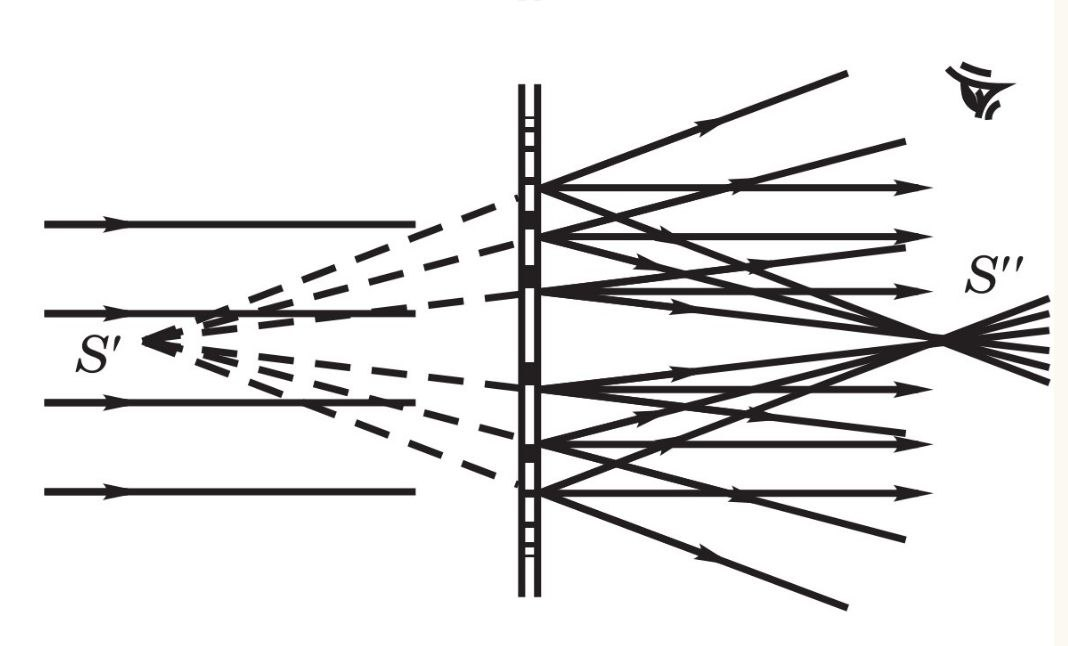
\includegraphics[width=\columnwidth]{images/point_s_t.jpeg}
	\caption{Голограмма точечного источника}
	\label{fig:point}
\end{figure}
\begin{equation}
	\begin{split}
		\Delta \phi(x) &= k \left( \sqrt{L^2 + x^2} - L \right) \approx \frac{k x^2}{2L} \\
		t(x) &\propto 1 + \cos\left( \frac{k x^2}{2L} \right)
	\end{split}
\end{equation}
При восстановлении плоской волной:
\begin{itemize}
	\item \textbf{Мнимое изображение}: на расстоянии $L$ за голограммой ($z' = -L$)
	\item \textbf{Действительное изображение}: на расстоянии $L$ перед голограммой ($z'' = L$)
\end{itemize}
При наклонной опорной волне ($\theta \neq 0$):
\begin{equation}
	\begin{split}
	\mathbf{k}_r = (k \sin\theta, 0, k \cos\theta) \quad \Rightarrow \\
	\quad \text{Смещение изображений: } \Delta x = \pm L \sin\theta
	\end{split}
\end{equation}

\subsection{Метод Денисюка (объёмные голограммы)}
\begin{figure}[H]
	\centering
	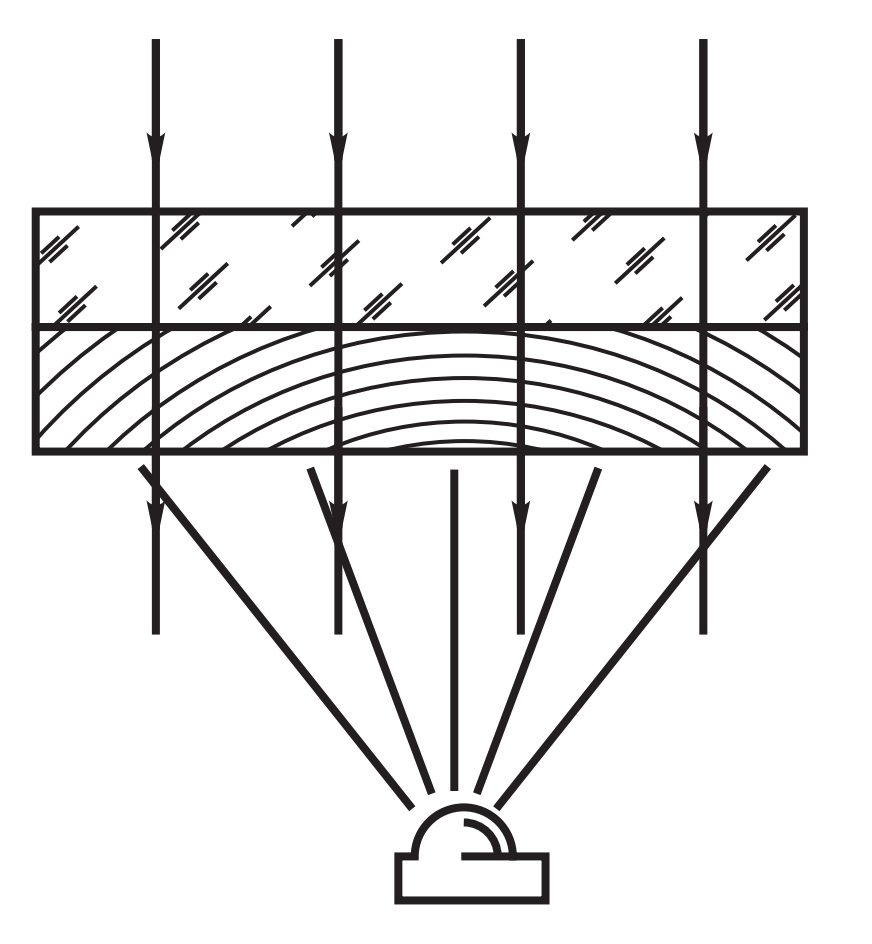
\includegraphics[width=\columnwidth]{images/den.png}
	\caption{Схема Денисюка}
	\label{fig:denisyuk}
\end{figure}
Опорная и предметная волны распространяются встречно (рис. \ref{fig:denisyuk}). Интерференция создаёт объёмную решётку с периодом:
\begin{equation}
	d = \frac{\lambda}{2n} \quad (n\text{ -- показатель преломления})
\end{equation}
Условие Брэгга для восстановления:
\begin{equation}
	2d \sin\alpha = \lambda_{\text{восст}}
\end{equation}
\textbf{Особенности:}
\begin{itemize}
	\item Восстанавливается только мнимое изображение
	\item Селективность по длине волны: $\lambda_{\text{восст}} \approx \lambda_{\text{записи}}$
	\item Возможно восстановление в белом свете
\end{itemize}

\subsection*{Разрешающая способность и размер голограммы}
Минимальный размер голограммы, использующий разрешение фотоэмульсии ($n$ [лин/мм]):
\begin{equation}
	a_{\min} = n \lambda L
\end{equation}
где $L$ -- расстояние до объекта. Размер изображения точки:
\begin{equation}
	b \approx \frac{\lambda}{\sin u}, \quad \sin u = \frac{a}{2L}
\end{equation}
\textbf{Требования к эмульсии:} 
\begin{itemize}
	\item Разрешение $> 3000$ лин/мм (для $\theta \sim 20^\circ$: $d \approx 2$ мкм)
	\item Линейная характеристика почернения
\end{itemize}

\section{Экспериментальная методика}
\textbf{Использованное оборудование:}
Проявитель OD1, тиосульфатный фотографический закрепитель (фиксаж), голографическая пластинка ПФГ-03М (5000 шт./мм)(\ref{subfig:plate}), установка для записи голограммы (\ref{subfig:construction1}, \ref{subfig:construction2}), лазерный модуль, безопасный свет (зеленный светодиод).
\begin{figure}[htbp]
	\centering
	\subfigure[пластинка]{
		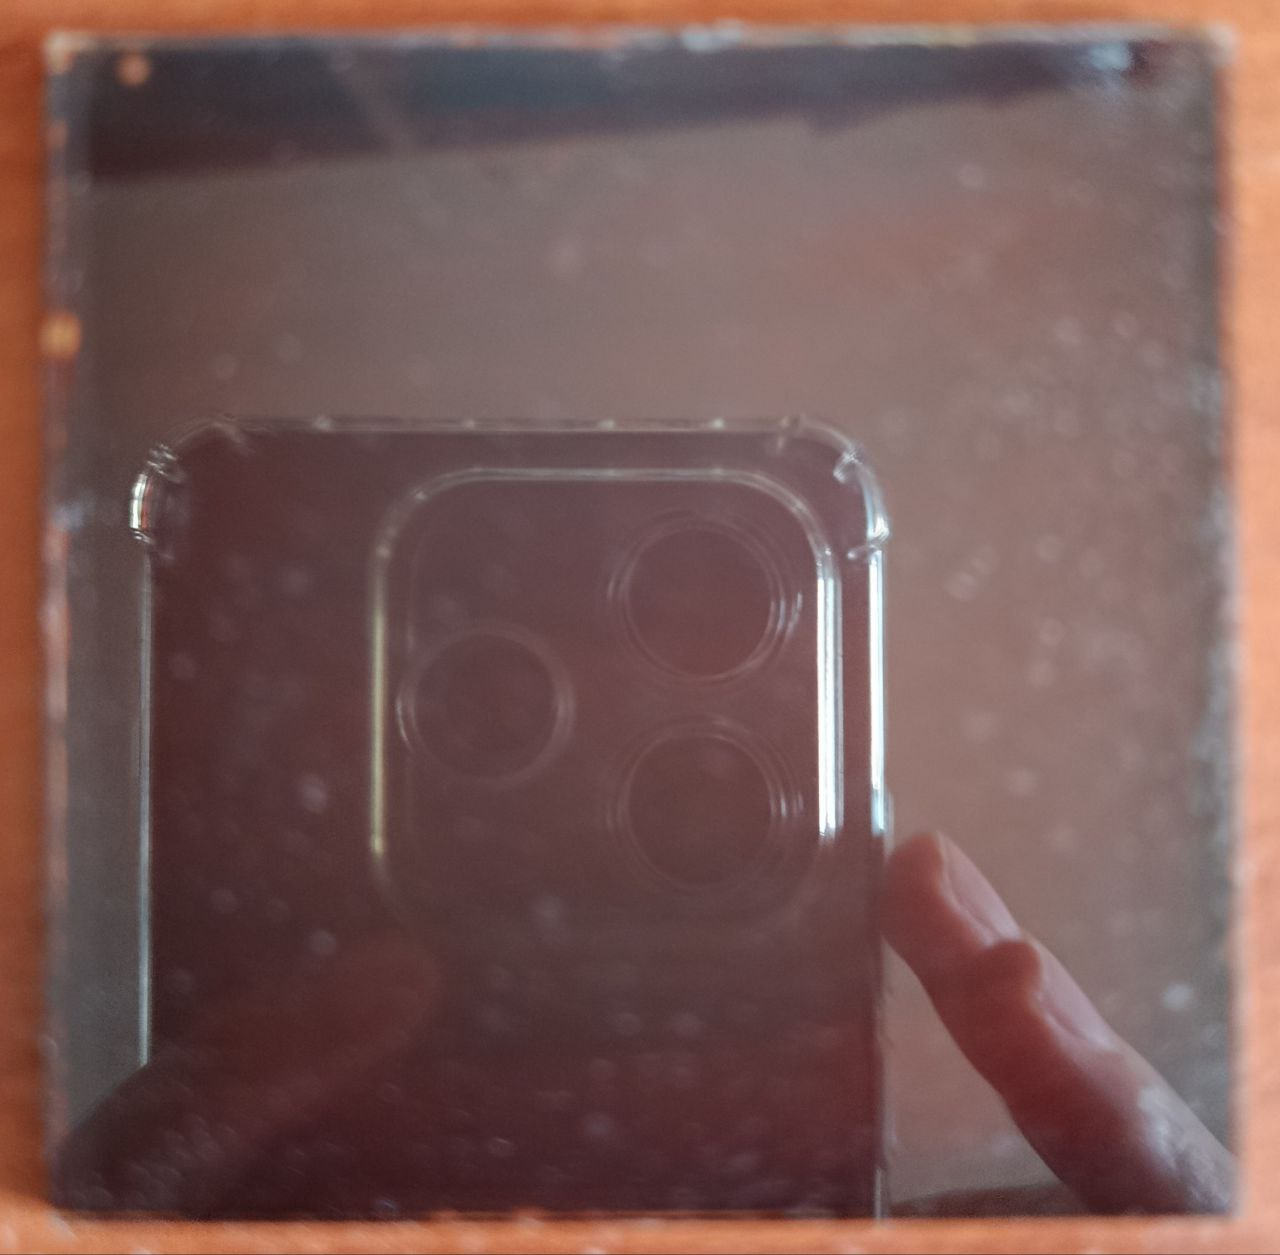
\includegraphics[width=0.45\columnwidth]{images/plate.jpeg}
		\label{subfig:plate}
	}
	\quad
	\subfigure[конструкция, вид сбоку]{
		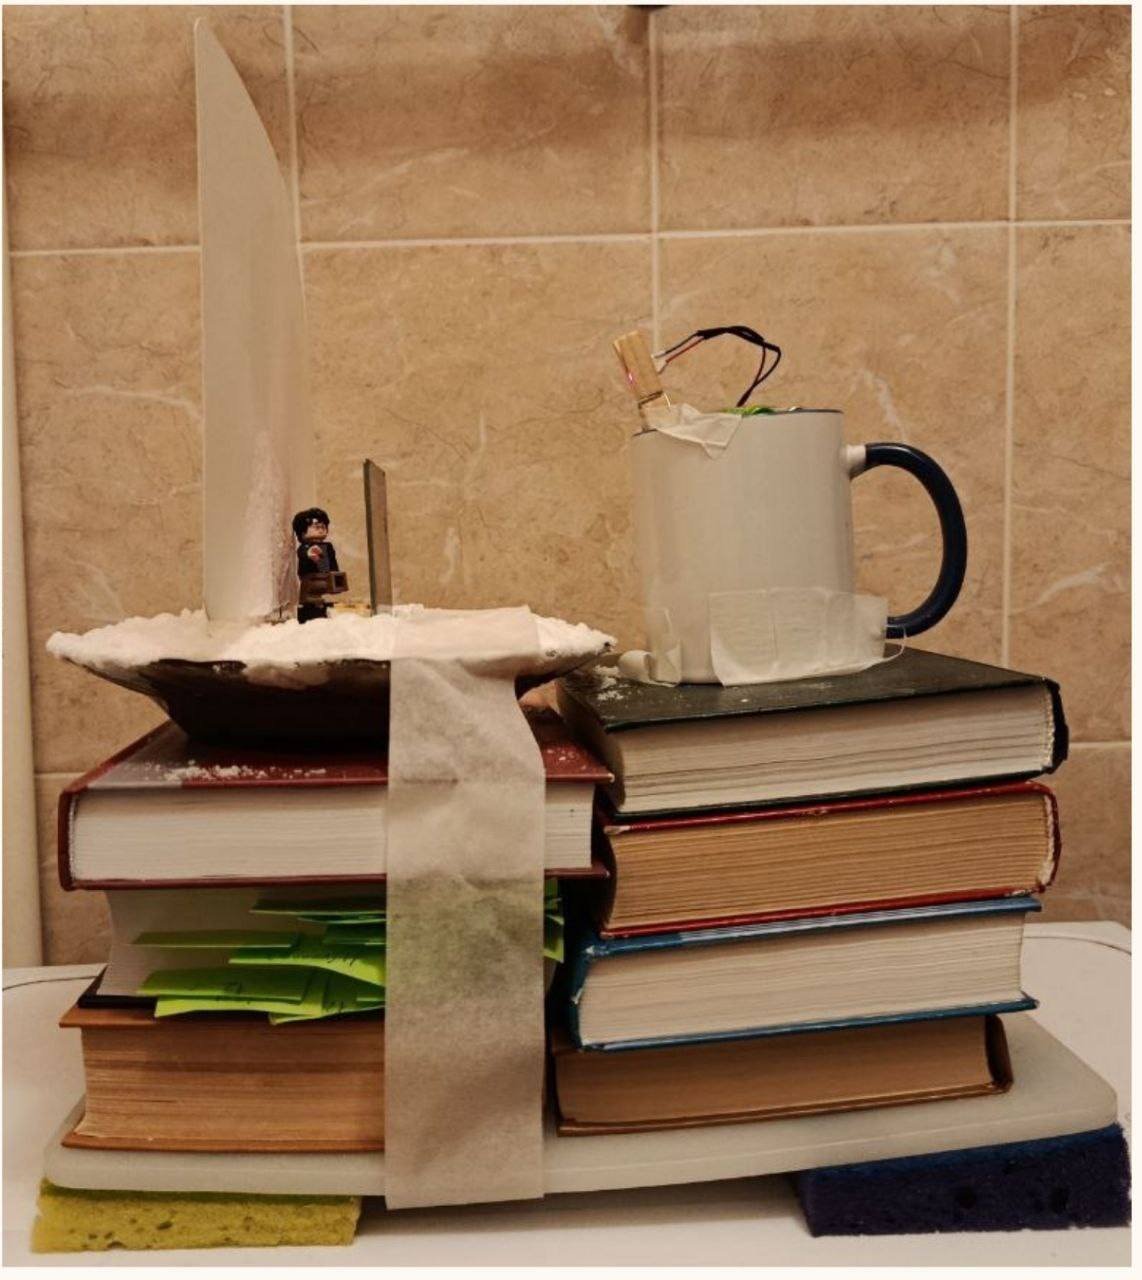
\includegraphics[width=0.45\columnwidth]{images/construction1.jpeg}
		\label{subfig:construction1}
	}
	\quad
	\subfigure[конструкция, вид сверху]{
		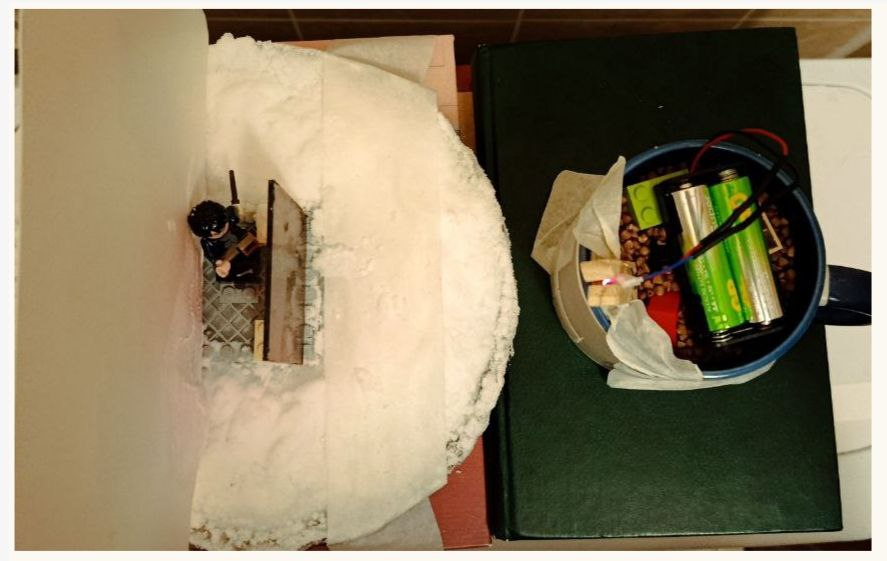
\includegraphics[width=\columnwidth]{images/construction2.jpeg}
		\label{subfig:construction2}
	}
	\label{fig:insruments}
	\caption{Инструменты использованные в работе}
\end{figure}
\textbf{Создание голограммы:}
\begin{enumerate}
	\item\textit{Подготовка реактивов.} Для записи голограммы нужно подготовить проявитель и фиксаж. Проявитель нужно смешать в одной из кювет с фильтрованной водой в отношении 1 к 3 (40 мл и 120 мл). Фиксаж просто налить в кювету. Также надо подготовить порядка литра чистой фильтрованной воды, для промывки голограммы. Вся использованная вода должна быть порядка 20 градусов цельсия. 
	\item\textit{Подготовка установки.} Для уменьшения вибраций, которые ухудшают записанную интерференционную картину, было:
	\begin{enumerate}
		\item Найдено тихое место (при этом было проверено, что в это время на улице не будет никаких сильных шумов).
		\item Пластинка и лазер установлены на тяжелую подставку, которая стоит на 4-х губках, которые гасят вибрации.
	\end{enumerate}
	Также при выборе места записи, важно отсутствие внешнего света, которое засветит пластину.
	\item\textbf{Запись голограммы.} (Все эти действия проводятся в полной темноте.)\\После разогрева лазера (примерно 10 минут), он освещает пластину на протяжение 10 секунд, после чего отключается (пример освещения голограммы лазером представлен на фото \ref{fig:laser_lighting}). Далее пластина помещается на 7 минут в проявитель. На протяжении всего этого времени кювета аккуратно покачивается, для лучшей проявки. После чего пластинка помещается на 2 минуты в фиксаж. \\
	(Далее действия можно проводить при свете.) На протяжении нескольких минут пластинка промывается холодной водой (лучше всего заранее подготовленной фильтрованной). Далее пластина сушится. Для того, чтобы на нейй налипло меньше пыли в процессе сушки, лучше всего ее чем-то накрыть (полотенцем)\\
	После высыхания при свете фонарика должна быть видна голограмма.
	\begin{figure}[H]
		\centering
		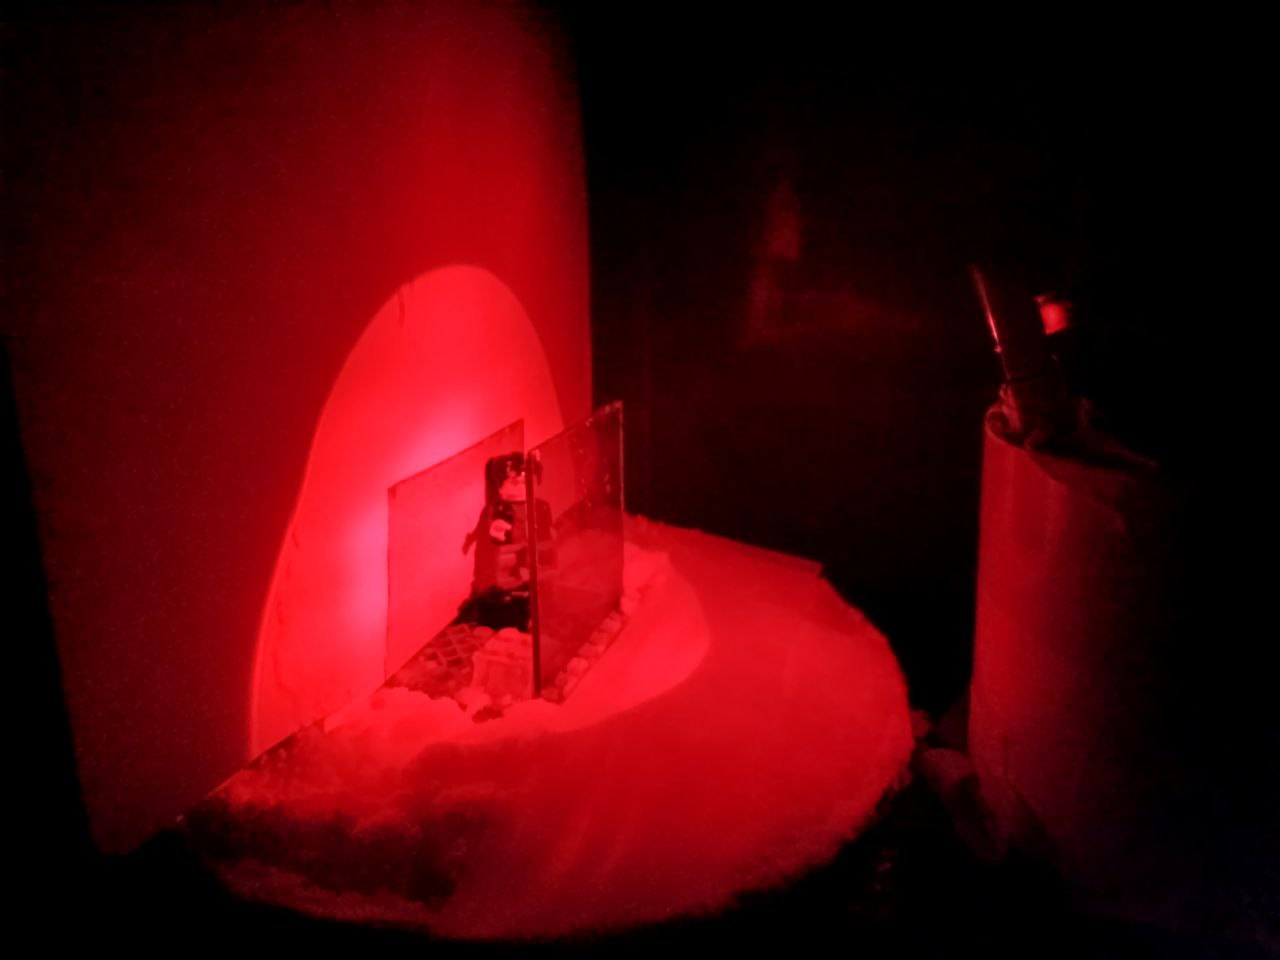
\includegraphics[width=0.45\textwidth]{images/laser_lighting.jpeg}
		\caption{Пример записи голограммы}
		\label{fig:laser_lighting}
	\end{figure}
\end{enumerate}
\section{Результаты}
\par Был опробовано три метода записи, которые отличаются расстановкой предмета и пластинки относительно лазера(\ref{fig:positions}). 
 \begin{figure}[H]
 	\centering
 	\subfigure[Пластинка находится над объектом, эмульсией к нему.]{
 		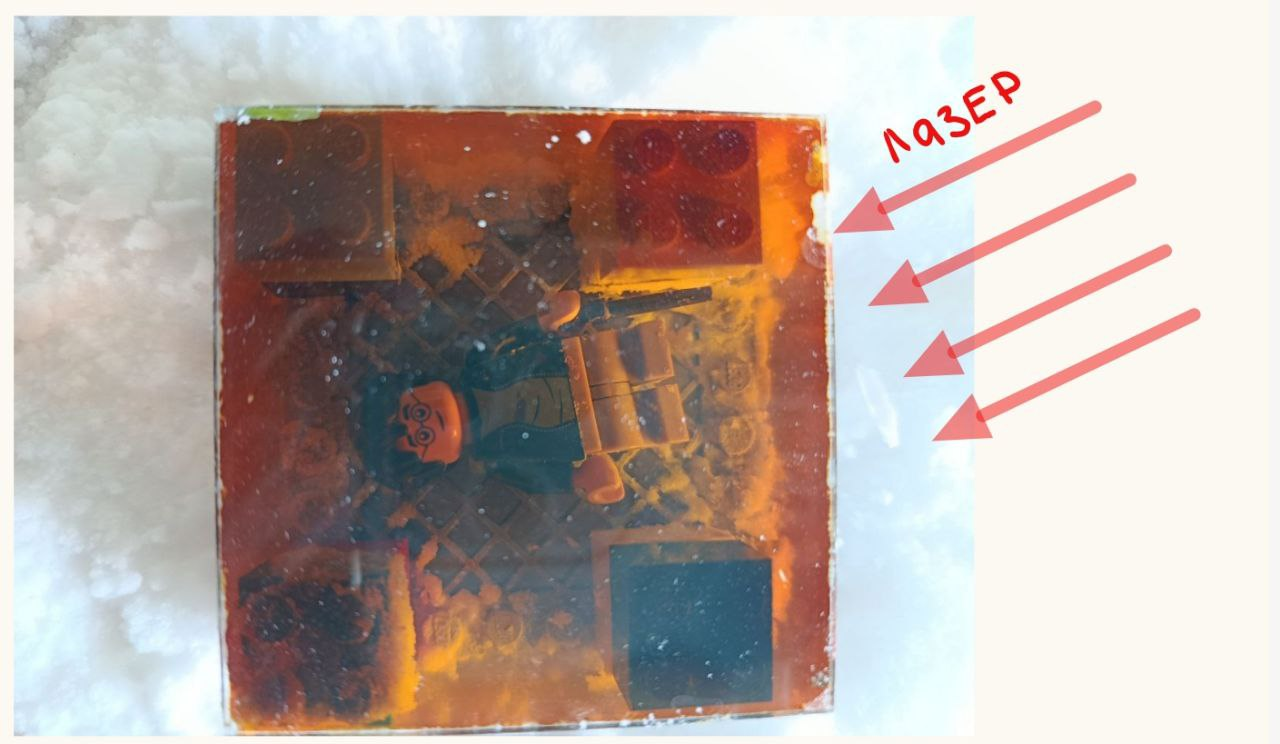
\includegraphics[width=\columnwidth]{images/pos2.jpeg}
 		\label{subfig:pos1}
 	}
 	\quad
 	\subfigure[Пластинка находится перед объектом, эмульсией к нему.]{
 		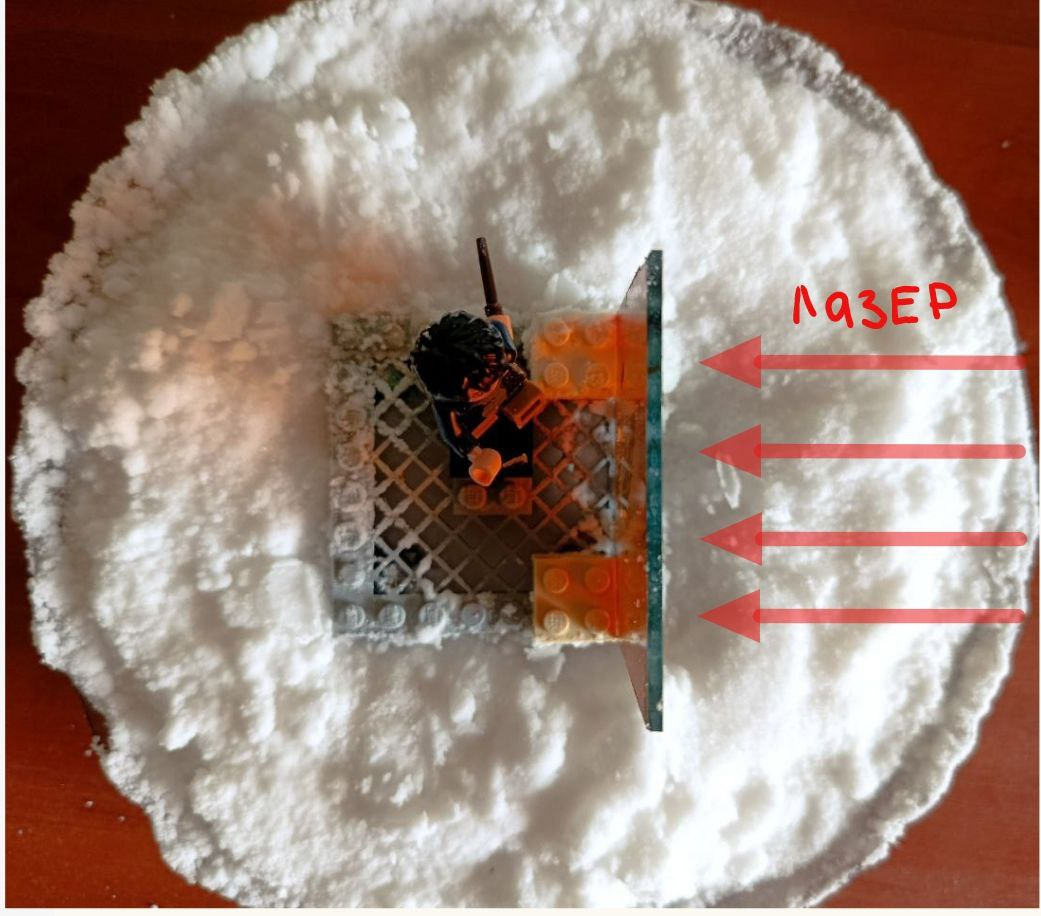
\includegraphics[width=0.45\columnwidth]{images/pos1.jpeg}
 		\label{subfig:pos2}
 	}
 	\quad
 	\subfigure[Палстинка находится рядом с объектом, повернута эмульсией к фигурке и лазеру.]{
 		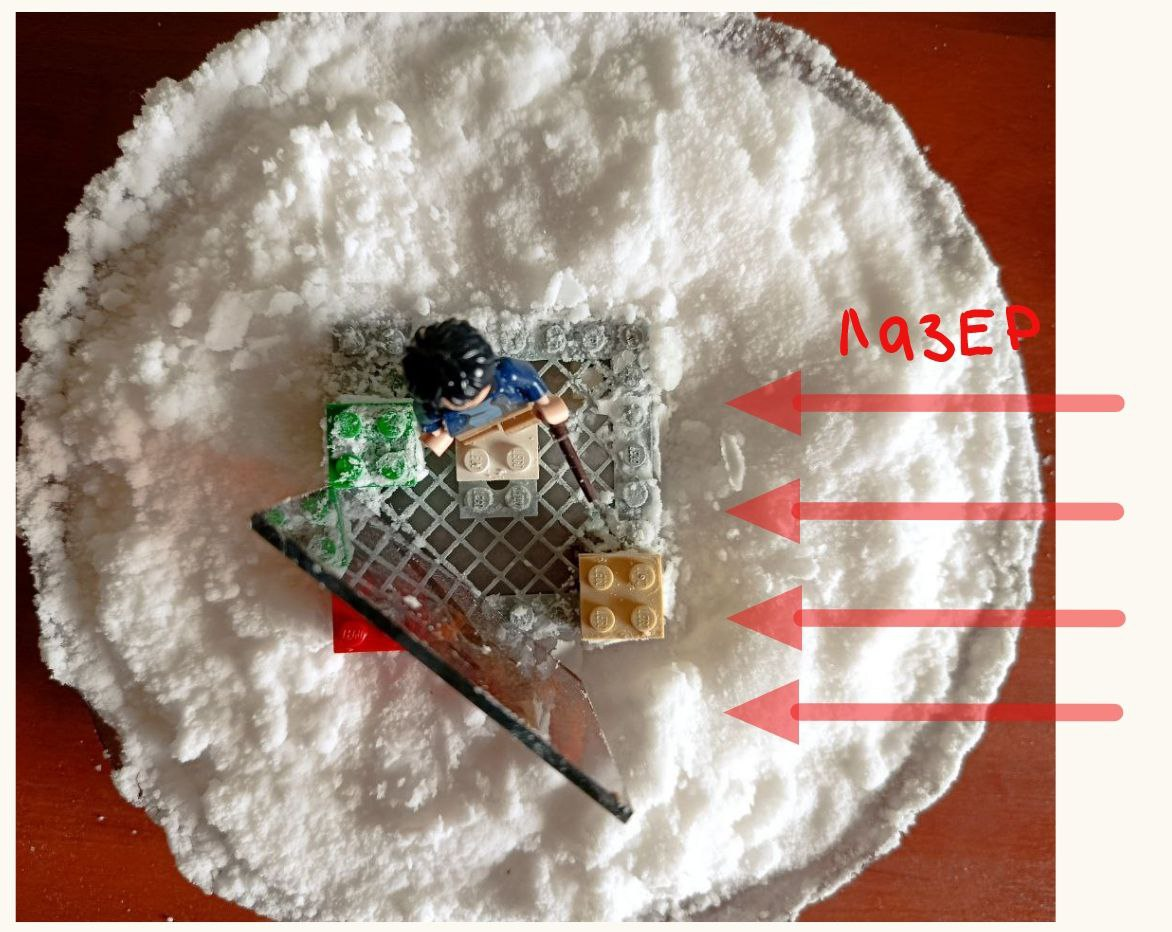
\includegraphics[width=0.45\columnwidth]{images/pos3.jpeg}
 		\label{subfig:pos3}
 	}
 	\label{fig:positions}
 	\caption{Расположения предмета и пластинки относительно лазера.}
 \end{figure}

Получилось что-то записать только первым способом.
\begin{figure}[H]
	\centering
	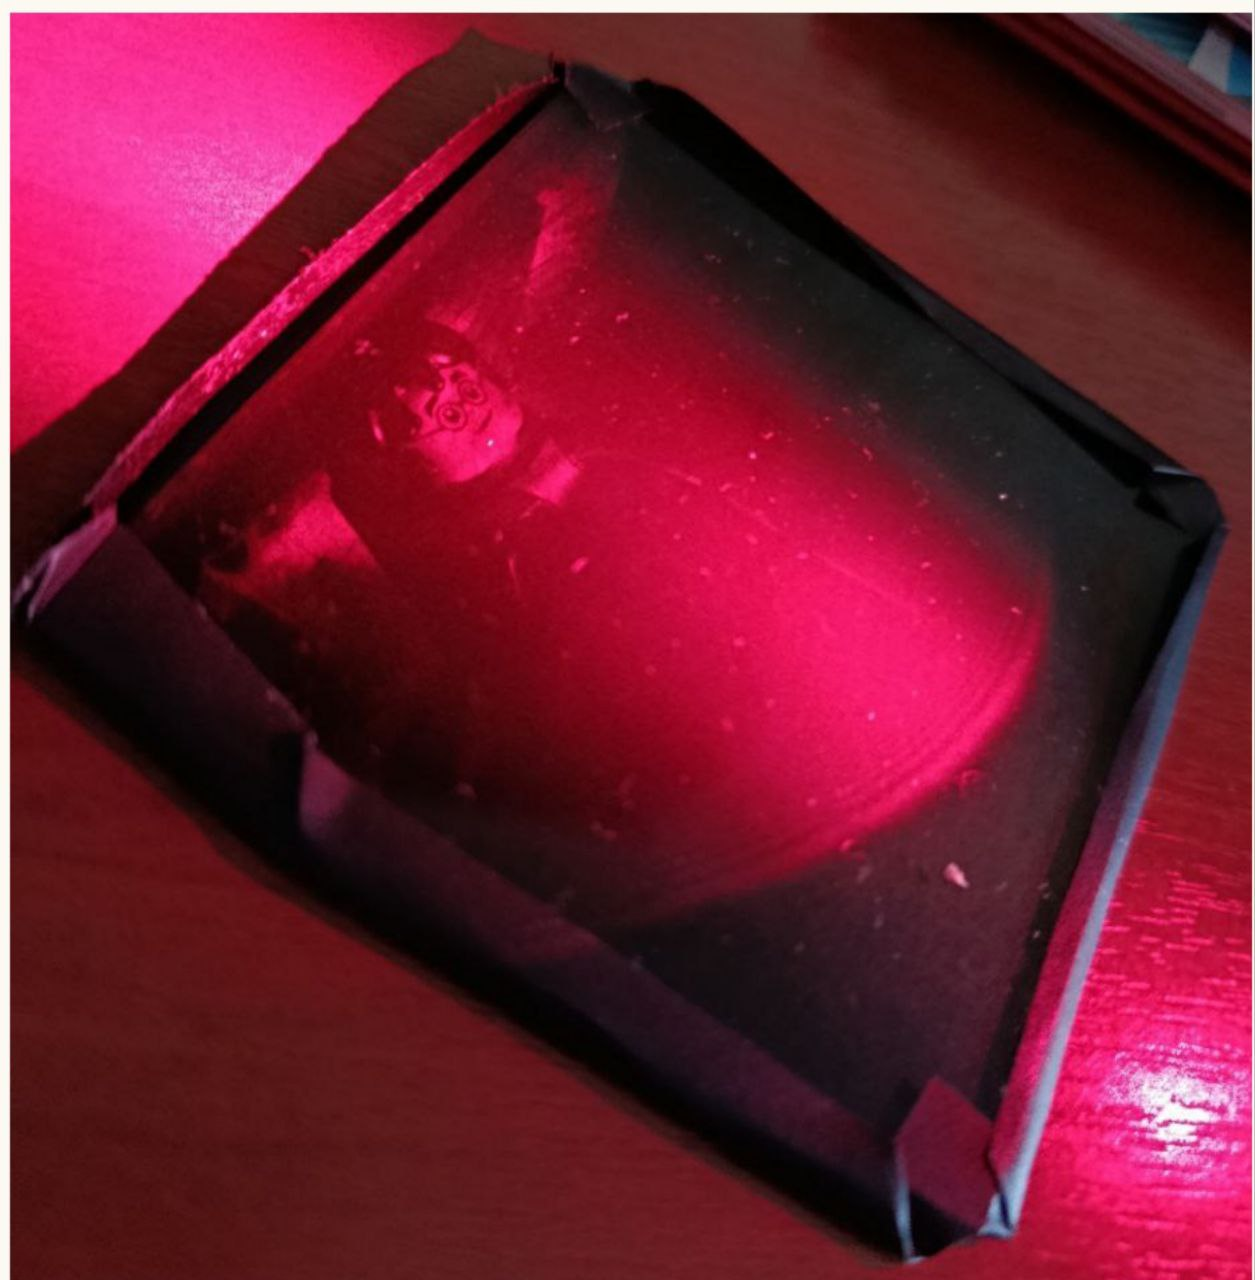
\includegraphics[width=0.45\textwidth]{images/real_hol.jpeg}
	\caption{Записанная голограмма.}
	\label{fig:result_hol}
\end{figure}
\par В процессе работы было выдвинуто несколько предположений, почему не получалось записать голограмму:
\begin{enumerate}
\item Лазер засвечивал пластину, поэтому он был передвинут подальше. Из-за этого времени в 10 секунд для записи стало не хватать, поэтому было попробовано несколько вариантов, первый из которых в 20 секунд представлен на фото, на нем видно, что пластина снова засвечена.
\begin{figure}[H]
	\centering
	\subfigure[Расположение объектов как на фото \ref{subfig:construction1}. Время экспозиции 10 секунд.]{
		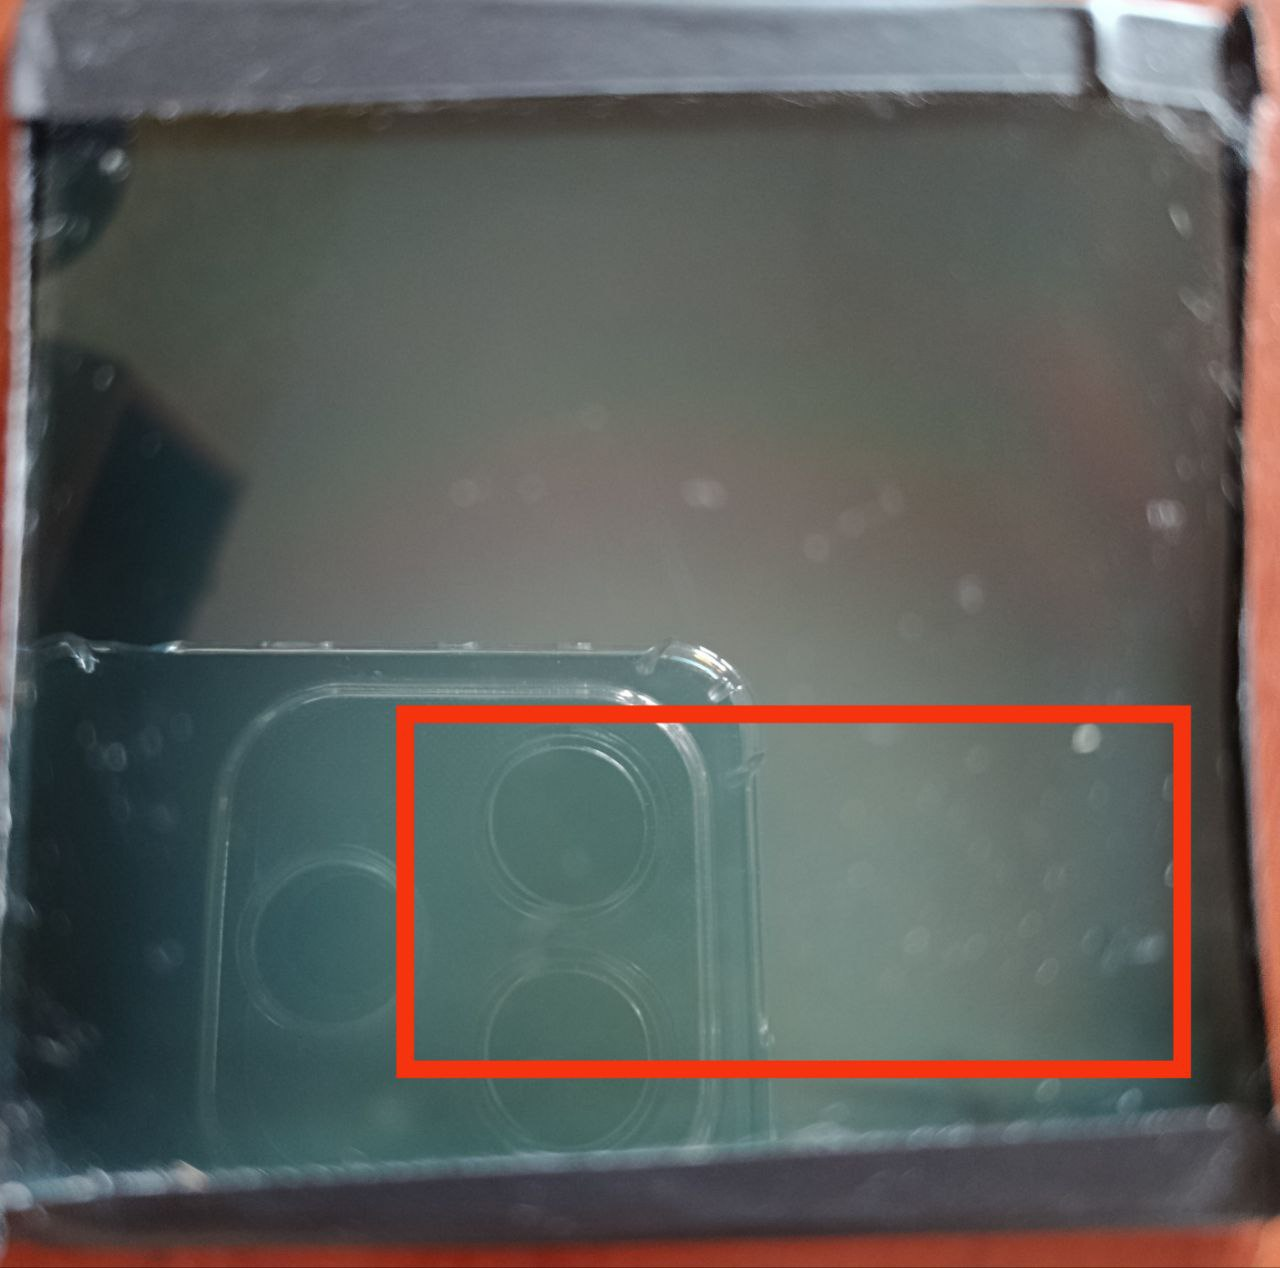
\includegraphics[width=\columnwidth]{images/light1.jpeg}
		\label{subfig:light1}
	}
	\quad
	\subfigure[Расстояние между пластиной и лазером увеличино в два раза. Время экспозиции 10 секунд.]{
		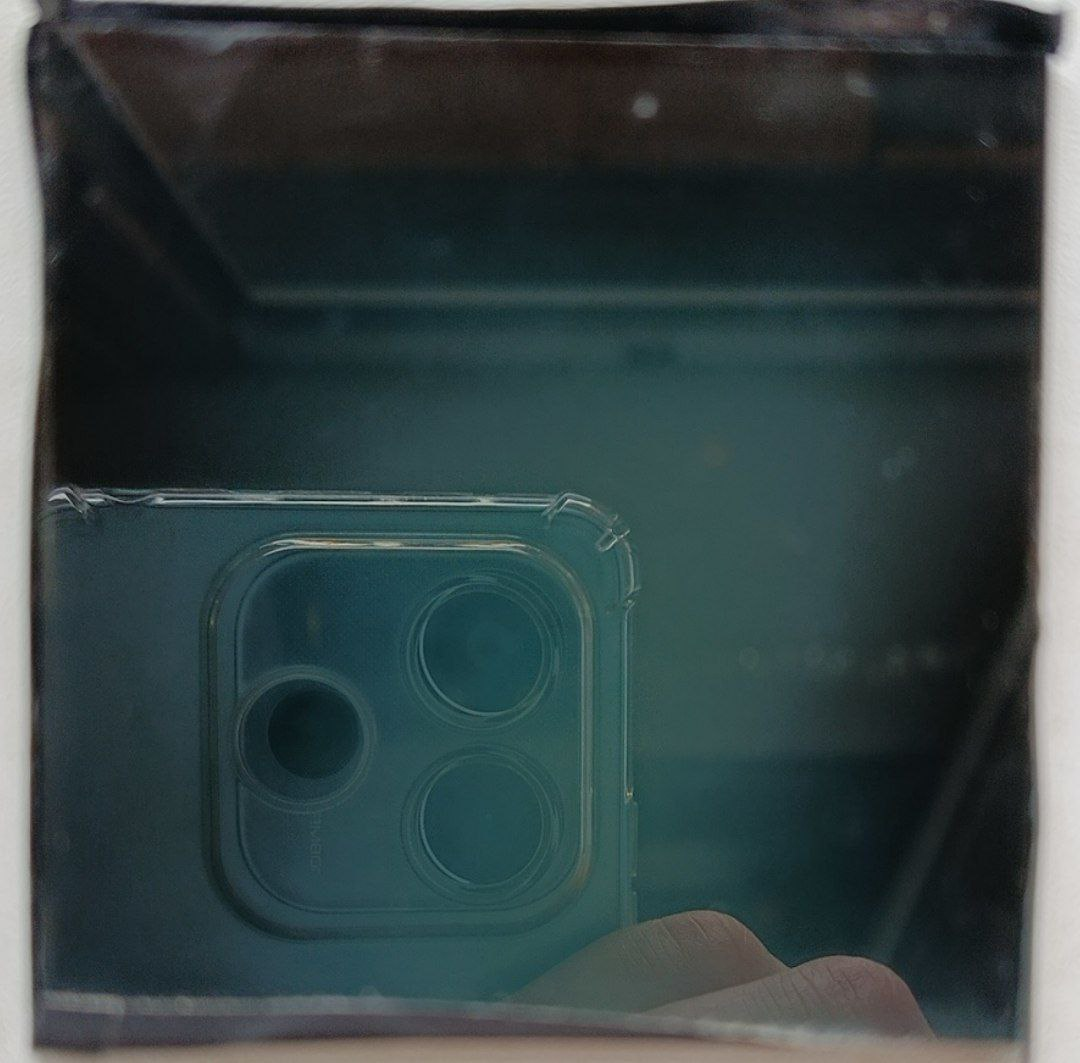
\includegraphics[width=0.45\columnwidth]{images/not_light.jpeg}
		\label{subfig:not_light}
	}
	\quad
	\subfigure[[Расстояние между пластиной и лазером увеличино в два раза. Время экспозиции 20 секунд.]{
		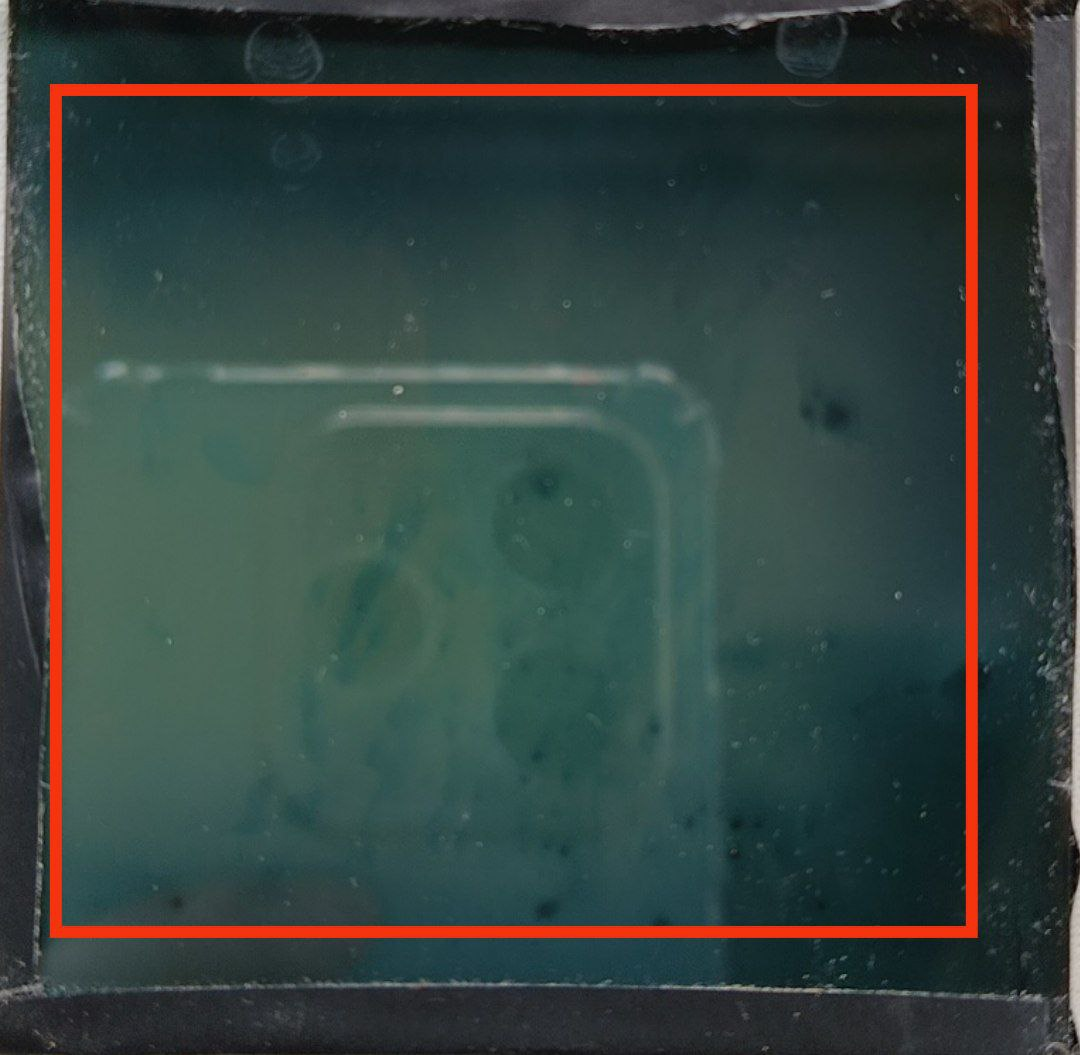
\includegraphics[width=0.45\columnwidth]{images/light2.jpeg}
		\label{subfig:light2}
	}
	\label{fig:light}
	\caption{Расположения предмета и пластинки относительно лазера.}
\end{figure}
\item Не хватает яркости отраженного света. Для этого была проведена запись без экрана (как на фото. \ref{subfig:pos2}), c полностью закрытым задним фоном (\ref{fig:closed_scene}), с белым и черным задним фоном (как на фото \ref{subfig:construction1}).
\begin{figure}[H]
	\centering
	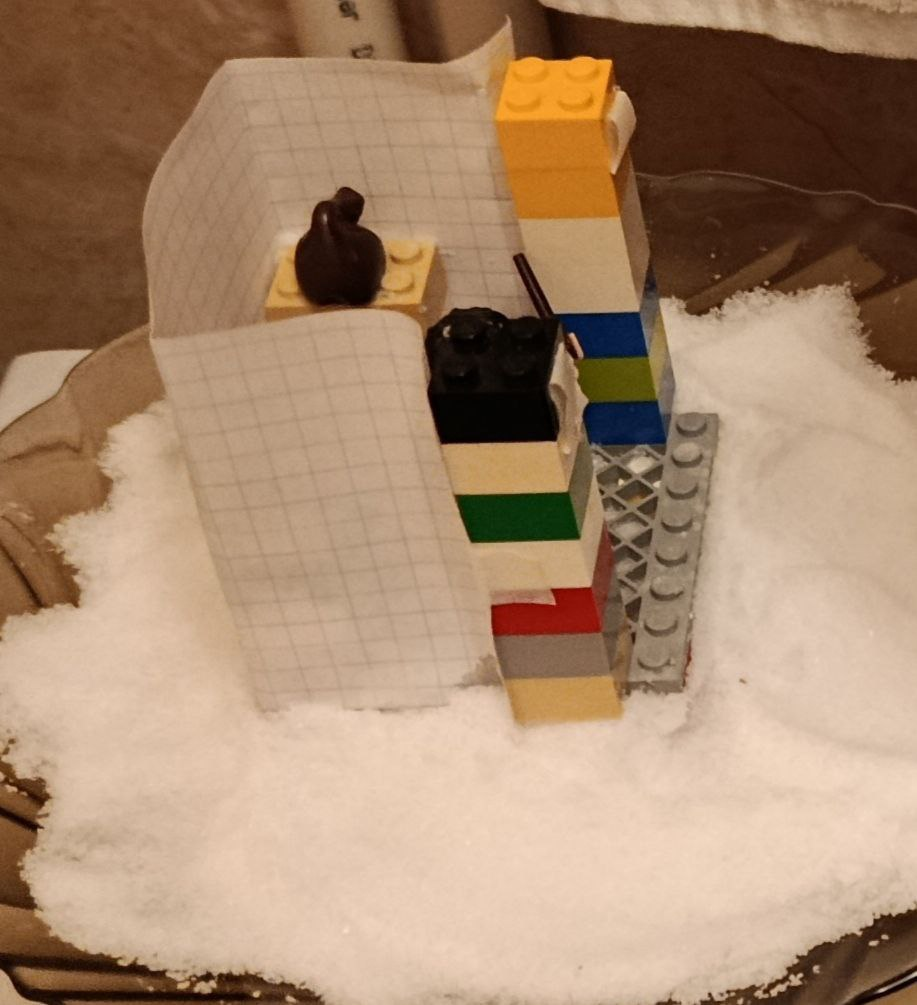
\includegraphics[width=0.45\textwidth]{images/closed_scene.jpeg}
	\caption{Задний фон со всех сторон закрыт белой бумагой.}
	\label{fig:closed_scene}
\end{figure}
\item Ещё одним предположением, почему не удавалось записать голограмму был радиус когерентности. А именно для этого лазера по заявлению продавца он является порядка 15-20 см, таким образом было уменьшено  расстояние между объектом и пластиной, чтобы для всех точек выполнялось это условие.
\item Для минимизации вибраций из вне, все записи проводились в середине ночи, когда не ходят электрички, а также по трубам не течет воды.
\end{enumerate}

\section{Описание реализации симуляции } 

\subsection{Архитектура проекта }

Проект состоит из нескольких модулей, каждый из которых отвечает за определённую часть симуляции:  
\begin{enumerate}
\item[-]\textbf{Генерация геометрии объекта}:  
Модуль `geometry` отвечает за задание формы объекта, разбиение его поверхности на сетку точек и проверку корректности геометрии.  

\item[-]\textbf{Запись голограммы}:  
Модуль `hologram\_prep` рассчитывает интерференционную картину, создаваемую объектным и опорным пучками, и сохраняет её в виде матрицы интенсивностей.  

\item[-]\textbf{Восстановление изображения}:  
Модуль `calculate\_visible\_field` позволяет восстанавливать видимое изображение объекта с учётом положения наблюдателя.  

\item[-]\textbf{Визуализация}:  
Используется библиотека OpenGL для отображения восстановленного изображения.  
\end{enumerate}
\subsection{Этапы работы} 
\begin{enumerate}
	\item Генерация геометрии объекта  
	
	Объект задаётся в виде набора поверхностей, каждая из которых представлена четырьмя вершинами:  
	\[
	\text{vertexes} = \{\{P_1, P_2, P_3, P_4\}, \dots\},
	\]  
	где \(P_i = (x, y, z)\).  
	
	Пример генерации объекта — плоского квадрата:  
	\begin{verbatim}cpp
		
		
	std::vector<std::vector<Point>> vertexes = {
	{ {0, 0, 0}, {1, 0, 0}, {0, 1, 0}, {1, 1, 0}}
	};
	obj_geometry geometry(1e-6, {100, 100}, 
			vertexes);
	geometry.calculate_points();
	\end{verbatim}
	\item Запись голограммы  
	Запись голограммы моделируется путём расчёта интерференционной картины. 
	\begin{verbatim}
std::string name_from = "file_with_geometry";
std::string name_to = 
	"file_where_to_save_intensity.txt";
double width = 10.0;
double height = 10.0;
double scale = 1e-6;
std::vector<unsigned int> np = {1024, 1024};
obj_plate plate(scale, np, width, height);
plate.readDataFromFile(name_from);
plate.calculate_intensity_matrix();
plate.saveIntensityToFile(name_to);
	\end{verbatim}
	\item Восстановление изображения  
	
	Восстановление голограммы выполняется методом быстрого преобразования Фурье (FFT). Использовалась библиотека `fftw3`. 
	\begin{enumerate}
		\item[-] \textbf{FFT} позволяет выделить пучок +1 порядка, содержащий информацию об объекте. 
		\item[-] Результат восстанавливается в виде матрицы интенсивностей, которая затем отображается.  
	\end{enumerate}
	Пример восстановленного изображения:
	\begin{verbatim}
		std::string name_from = "file_with_intensity";
		v_plate = obj_visible_plate(1e-6);
		v_plate.read_intensity_matrix(name_from);
		...
		while(...){ //main loop
			...
			v_plate.update_visible_matrix(cameraPos.x,
			 cameraPos.y, cameraPos.z);
			...
		}
	\end{verbatim}	
\end{enumerate}
\subsection{Результаты моделирования}
(Получилось мало чего, но мы честно пытались, а еще мысли что делать дальше)
\begin{figure}[htbp]
	\centering
	\subfigure[интерференционная картина для точеченого источника]{
		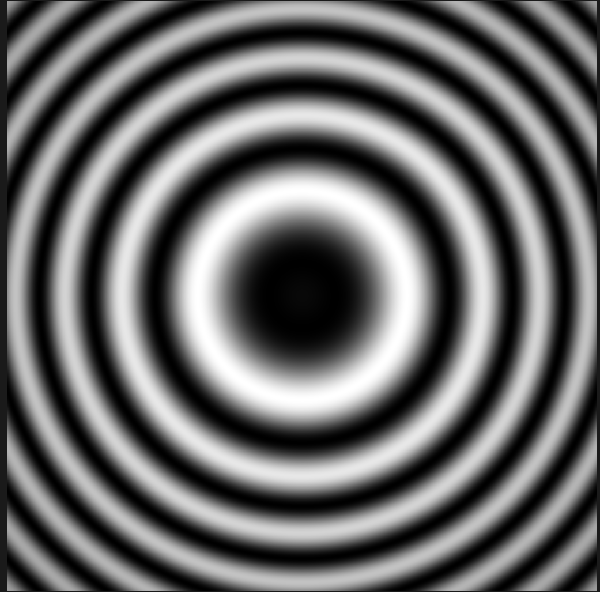
\includegraphics[width=0.21\textwidth]{images/point_interf.png}
		\label{subfig:point_interf}
		%\caption{fig1}
	}
	\quad
	\subfigure[]{
		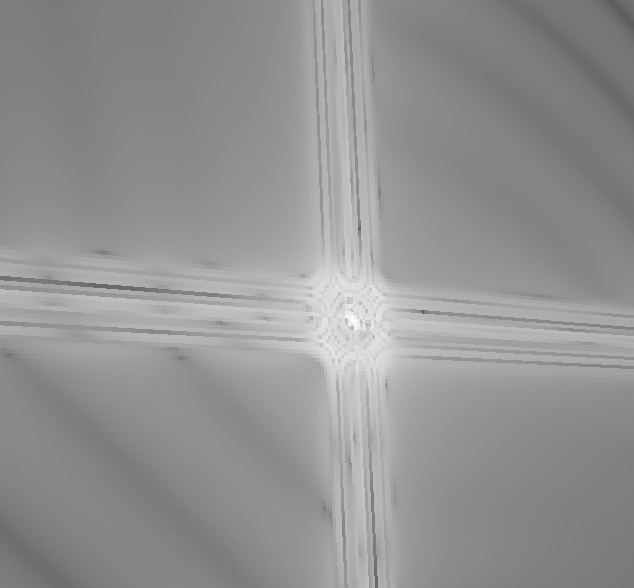
\includegraphics[width=0.21\textwidth]{images/point1.png}
		\label{subfig:point1}
		%\caption{fig1}
	}
	\quad
	\subfigure[]{
		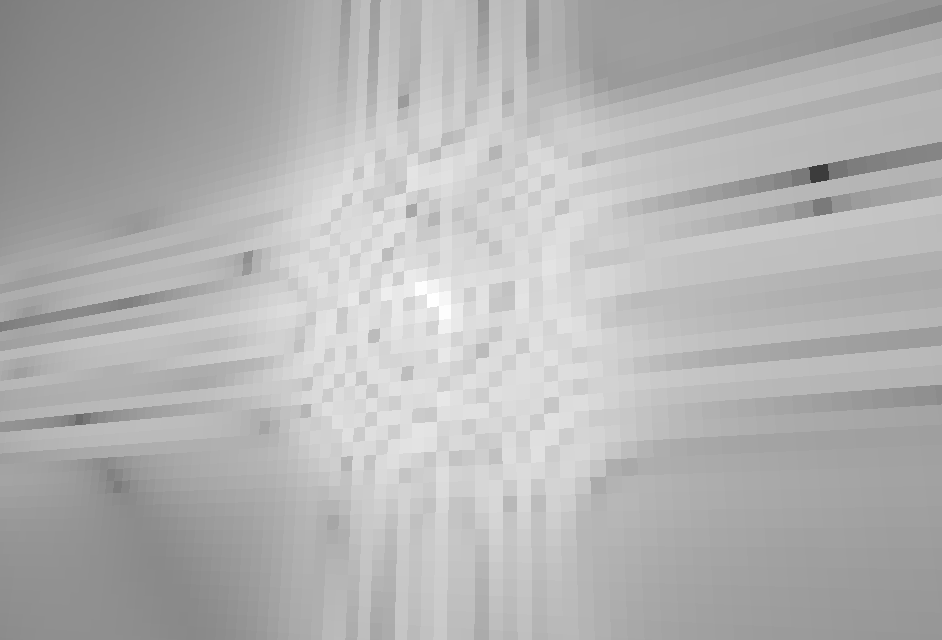
\includegraphics[width=0.21\textwidth]{images/point2.png}
		\label{subfig:point2}
	}
	\quad
	\subfigure[]{
		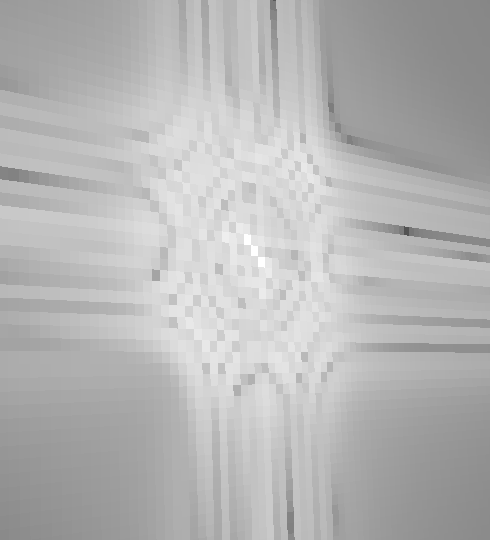
\includegraphics[width=0.21\textwidth]{images/point4.png}
		\label{subfig:point3}
	}
	\caption{Интерференционная картина, которая бы была на транспаранте и изображение точеной голограммы с разных ракурсов (можно заметить, что немного картины интенсивностей, который бы видел человеческий глаз меняются)}
	\label{fig:point_hologram}
\end{figure}
\begin{figure}[htbp]
	\centering
	\subfigure[геометрия, расчитанная в этом варианте]{
		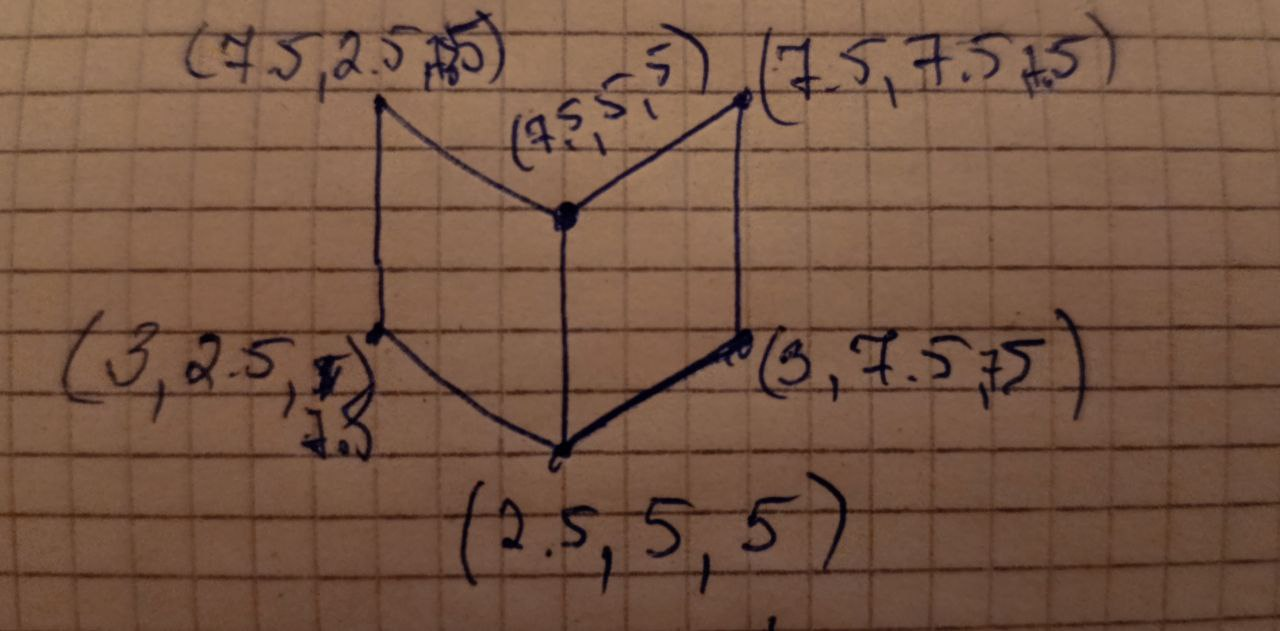
\includegraphics[width=0.45\columnwidth]{images/book.jpeg}
		\label{subfig:book}
		%\caption{fig1}
	}
	\quad
	\subfigure[интерференционная картина для точеченого источника]{
		
\includegraphics[width=0.45\columnwidth]{images/sq_interf.png}
		\label{subfig:sc_interf}
		%\caption{fig1}
	}
	\quad
	\subfigure[]{
		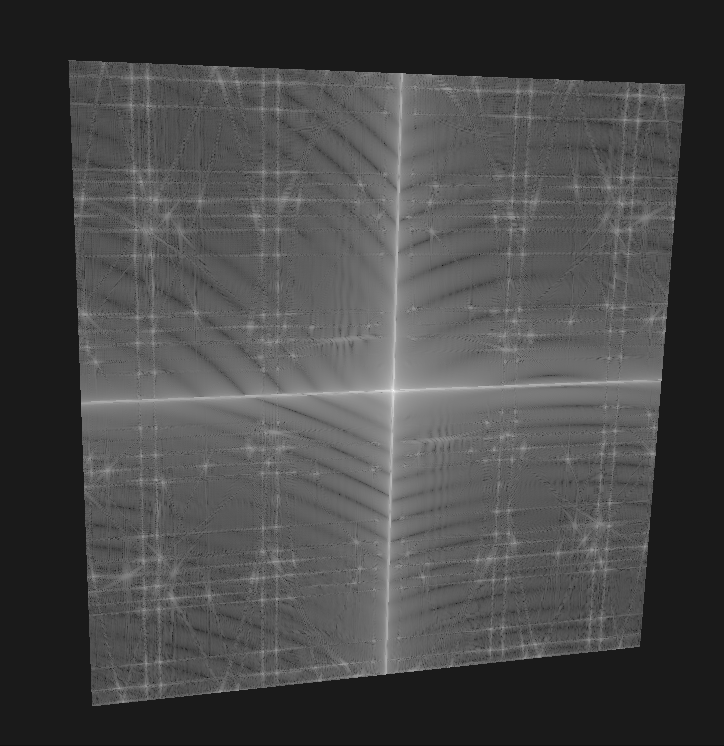
\includegraphics[width=0.45\columnwidth]{images/screen1.png}
		\label{subfig:screen1}
	}
\quad
\subfigure[]{
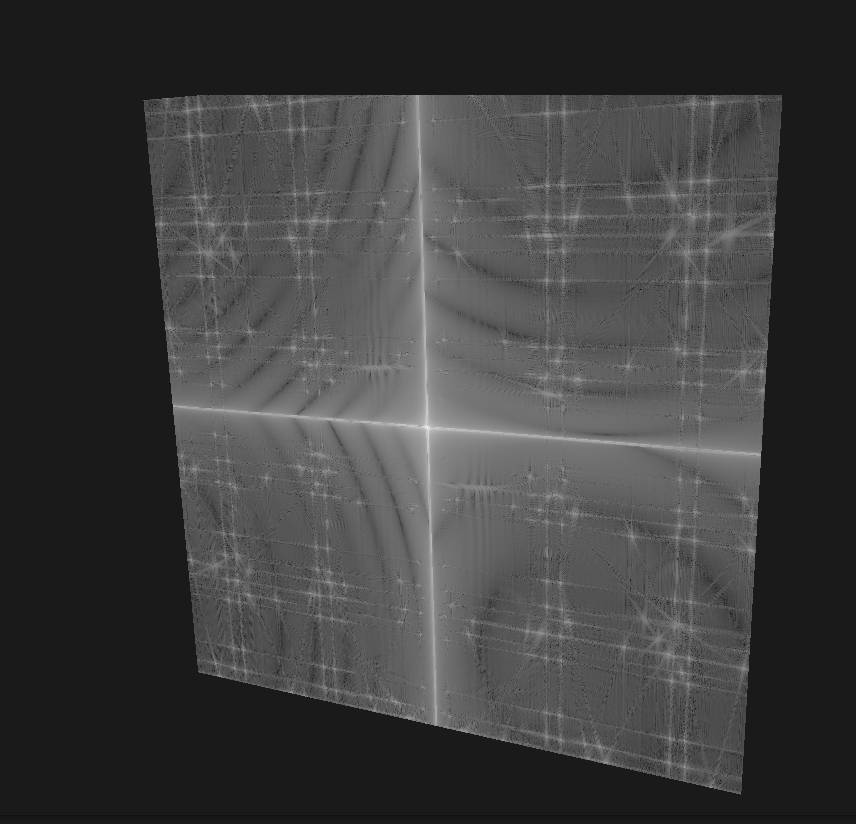
\includegraphics[width=0.45\columnwidth]{images/sq_2.png}
\label{subfig:sq_2}
}
	\caption{Геометрия, интерференционная картина, которая бы была на транспаранте и изображение объемной голограммы с разных ракурсов (можно заметить, что немного картины интенсивностей, который бы видел человеческий глаз меняются)}
	\label{fig:book_hol}
\end{figure}
\section{Обсуждение результатов}
\par При записи голограммы, получилось что-то записать и потом это увидеть только один раз. Есть несколько вариантов почему мало что получилось:
\begin{enumerate}
	\item Пластинки плохого качества (они были заказные);
	\item Лазер в процессе работы ломался, поэтому его приходилось чинить (возможно светить он начал, но уже не с теми характеристиками);
	\item Возникали шумы (вибрации), не учтенные пр работе;
	\item Некачественные реактивы.
\end{enumerate}
\par При моделировании так же возникло много проблем, вот некоторые предположения почему так вышло:
\begin{enumerate}
	\item Где-то появилась ошибка в задании фазы;
	\item Не так подобрана нормировка рассчитанных значений.
\end{enumerate}
\section{ Итоги и выводы  }
\begin{enumerate}
	\item Записна голограмма объемного источника;
	\item Выявлен ряд причин, почему не получалось записать голограмму;
	\item Реализована программная модель записи и восстановления голограммы.
\end{enumerate}
\section{Ссылки на литературу}  

1. Hecht, E. \textbf{Optics}, Fifth Edition. Pearson Education, 2017.  
2. Бутиков Е. И. \textbf{Оптика: Учебное пособие}. 3-е изд. Санкт-Петербург: Лань, 2016.  

\section{Приложения}  
Код проекта расположен по \href{https://github.com/ArinaLuzgina/holographySimulation}{ссылке}.
\end{document}
